\chapter{状態推定の不確かさを考慮した\\障害物の回避動作} \label{chapter:method}
本章では, 状態推定の不確かさを考慮した障害物の回避動作を生成する手法について述べる. 
\ref{section:一般的な回避}節では, 現在一般的行われているような移動ロボットの回避行動について述べる. 
\ref{section:method overview}節では, 提案手法の概要について簡単に述べる. 
\ref{section:障害物}節では, 本論文において回避を行う障害物の定義を述べる. 
\ref{section:価値関数}節では, 提案手法やPFC法に必要となる, 価値関数を計算する方法について述べる. 
\ref{section:回避重み}節では, 提案する手法についての詳細を述べる. 


%%%%%%%%%%%%%%%%%%%%%%%%%%%%%%%%%%%%%%%%%%%%%%%%%%%%%%%%%%%%%%%%%%%%%%%%%%%%%%%%
\section{一般的な行動決定による障害物回避} \label{section:一般的な回避}
多くの移動ロボットによる行動決定では, 図\ref{fig:一般的な行動決定}に示すように, 
信念分布の中で最も確率の高い姿勢のみを行動決定に利用する. 
MCLで姿勢推定を行うロボットであれば, 信念分布を近似するパーティクルの分布の中で, 
最も重みの大きいパーティクルを利用する. 
ロボットは推定した姿勢の移動距離が最短となるように障害物を回避する経路を辿りゴールへと向かう. 
つまり, 行動決定は分布の大きさや形が考慮されずに行われるということになる. 

\begin{figure}[h]
  \begin{center}
    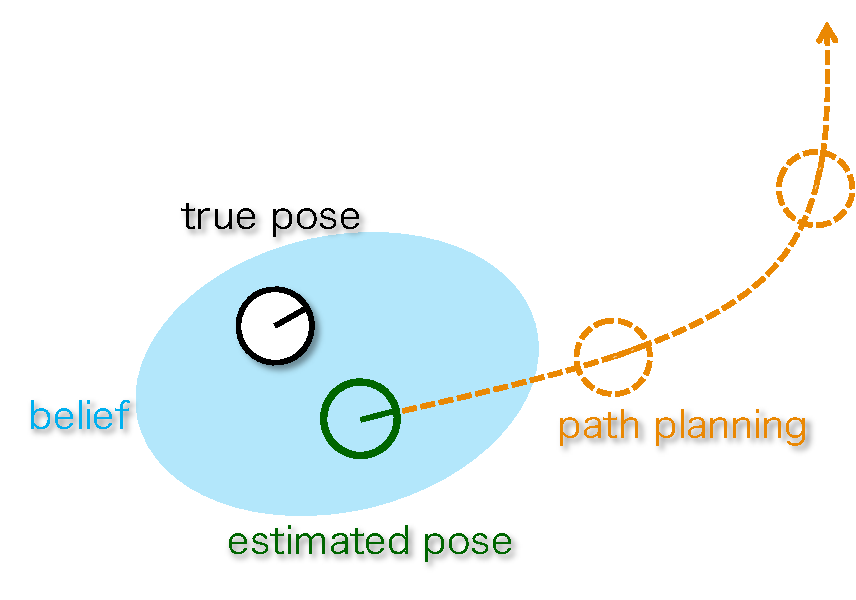
\includegraphics[width=10cm, ]{一般的な行動決定.pdf}
    \caption{Path planning for general mobile robot}
    \label{fig:一般的な行動決定}
  \end{center}
\end{figure}

\begin{figure}[h]
  \begin{center}
    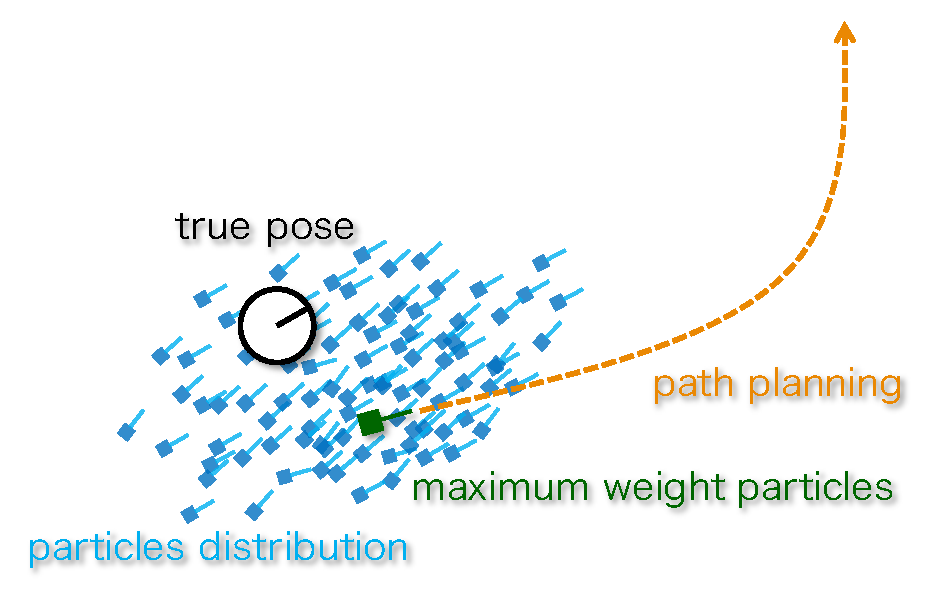
\includegraphics[width=10cm, ]{一般的な行動決定MCL.pdf}
    \caption{Path planning for a robot that localization using MCL}
    \label{fig:一般的な行動決定MCL}
  \end{center}
\end{figure}

しかし, この方法には障害物への衝突リスクが伴うことが考えられる. 
例えば, 図\ref{fig:障害物回避タスクの例}に示すように, 
ロボットが障害物を一つ回避しゴールへと向かう経路を移動する場合について考える. 
一般的な行動決定では, 図\ref{fig:一般的な障害物回避}に示すように, ロボットは推定した一つの姿勢が障害物を回避するように行動する. 
しかし, もし黒色で示されている真のロボットが, 緑色で示されている推定値よりもインコース側に存在するような状況では, 
ロボットの障害物衝突が考えられる. 
これを防ぐためには, 最高確率の推定値のみではなく, 信念分布全体を使用して行動決定を行うことが有効となる. 

\begin{figure}[h]
  \begin{center}
    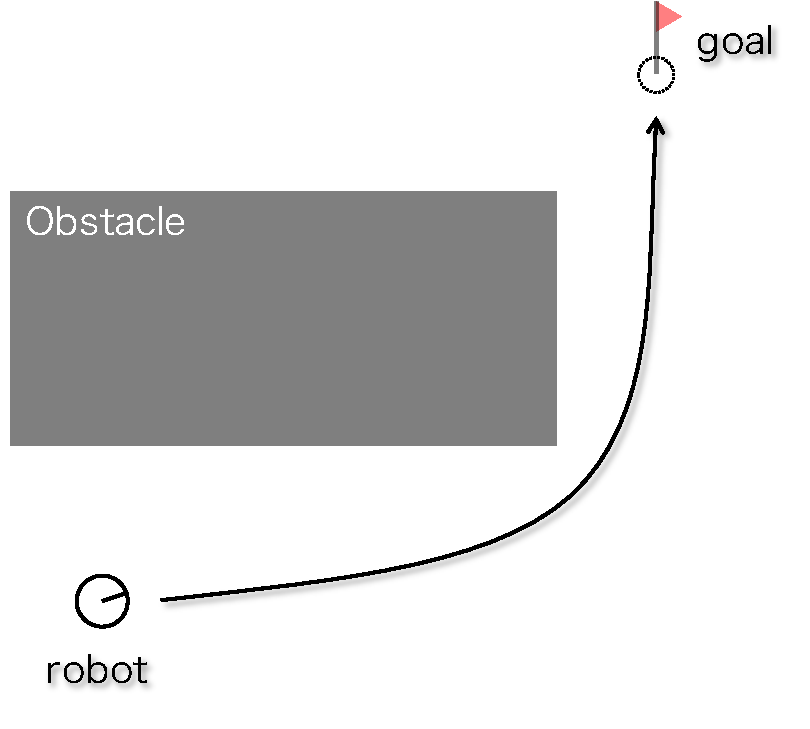
\includegraphics[width=10cm, ]{障害物回避タスクの例.pdf}
    \caption{Example of a task to avoid obstacle}
    \label{fig:障害物回避タスクの例}
  \end{center}
\end{figure}

\begin{figure}[h]
  \begin{center}
    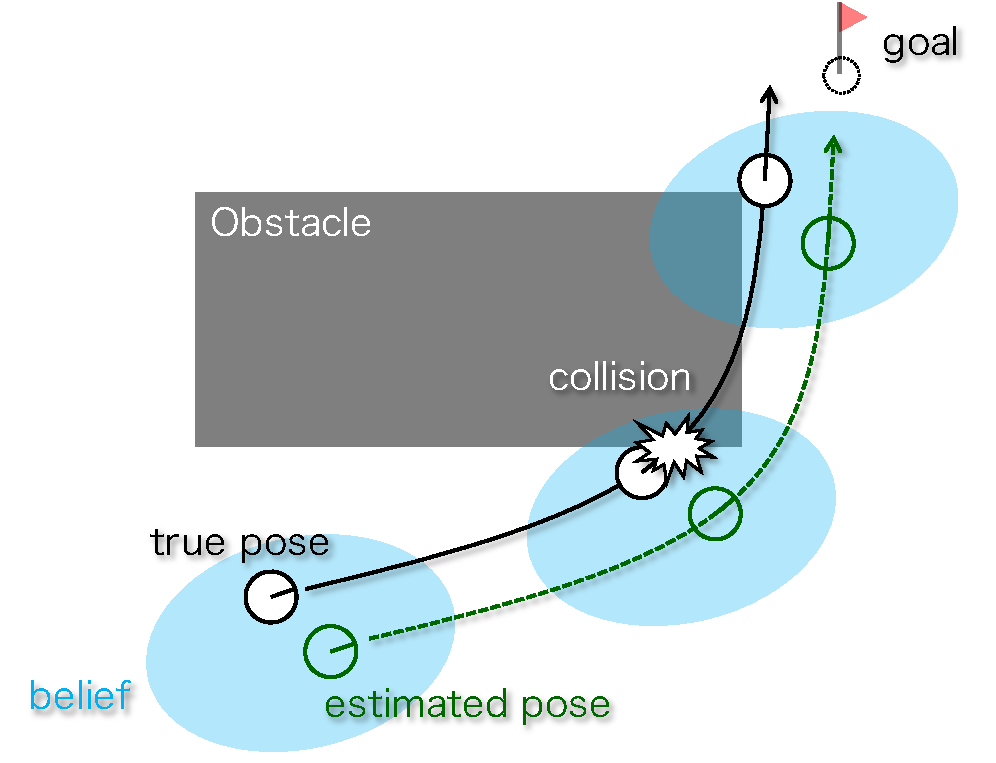
\includegraphics[width=12cm, ]{一般的な障害物回避.pdf}
    \caption{Collision risk due to general obstacle avoidance behavior}
    \label{fig:一般的な障害物回避}
  \end{center}
\end{figure}


%%%%%%%%%%%%%%%%%%%%%%%%%%%%%%%%%%%%%%%%%%%%%%%%%%%%%%%%%%%%%%%%%%%%%%%%%%%%%%%%
\section{提案手法の概要} \label{section:method overview}
本論文では, \ref{section:一般的な回避}節で述べたような障害物衝突のリスクを, 
不確かさを考慮した障害物の回避行動を生成する. 
移動ロボットの行動決定に信念分布全体を利用し, 推定の不確かさを考慮した行動を行わせる. 
図\ref{fig:不確かさを考慮した障害物回避}に示すように, 
信念分布全体が障害物を回避するようにロボットを動作させる. 
こうすることで, ロボットの自己位置推定が正しく行われており真の姿勢がパーティクルの分布内に存在すような場合, 
ロボットが障害物に侵入するのを防ぐことを可能にする. 
本手法では, MCLで姿勢推定をする移動ロボットを想定し, 
ロボットの信念分布を近似するパーティクルの分布全体が, 障害物外を移動するようにロボットを動作させる. 

\begin{figure}[h]
  \begin{center}
    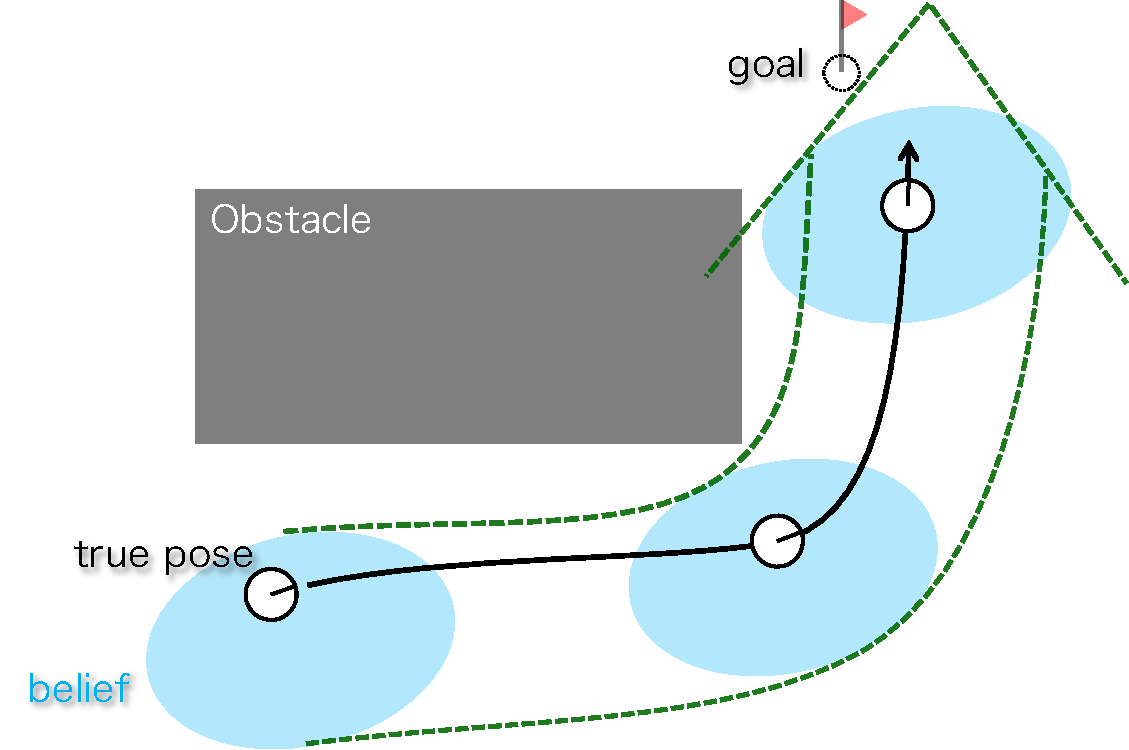
\includegraphics[width=12cm, ]{不確かさを考慮した障害物回避.pdf}
    \caption{Obstacle avoidance considering uncertainty.}
    \label{fig:不確かさを考慮した障害物回避}
  \end{center}
\end{figure}

\ref{section:PFC法}節で述べたPFC法に変更を加えることで, この動作を実現する. 
オフラインフェーズでは, 通常のPFC法同様に, 観測に関する不確かさがない前提でMDP問題を解き最適価値関数を計算する. 
変更は, 実際にロボットの行動決定を行うオンラインフェーズでの行動評価の式に行う. 
PFC法では, パーティクル全体の状態価値の合計の期待値が最大となる行動を選択する. 
この期待値計算の際に, パーティクルの現在の状態価値に応じて重み付けを行う. 
つまり, ゴール付近のパーティクルが行動決定に与える影響を強くすることで, ゴール探索動作を実現している. 

本手法では, 通常のPFC法に加え, 障害物付近のパーティクルが行動決定に与える影響も強める処理を追加する. 
図\ref{fig:手法概要}に示すように, 次ステップの行動で障害物内に侵入する可能性があるパーティクルが, 
行動決定に与える影響度を一時的に大きくすることで, 回避動作を行わせる. 
これにより, パーティクルの分布全体が障害物を避けるような動作を行わせるとともに, 
PFC法の利点である, ゴール付近で分布をゴールに流し込むような探索動作を行うことが可能となる. 

\begin{figure}[h]
  \begin{center}
    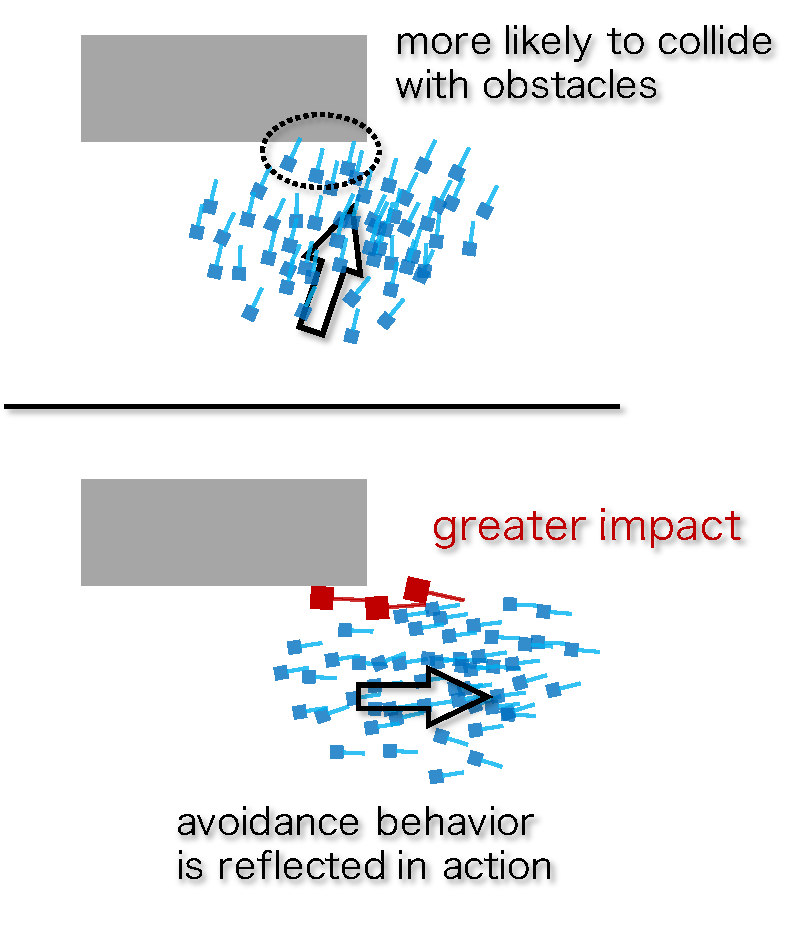
\includegraphics[width=12cm, ]{手法概要.pdf}
    \caption{Overview of the method}
    \label{fig:手法概要}
  \end{center}
\end{figure}


%%%%%%%%%%%%%%%%%%%%%%%%%%%%%%%%%%%%%%%%%%%%%%%%%%%%%%%%%%%%%%%%%%%%%%%%%%%%%%%%
\section{本論文における障害物} \label{section:障害物}
本節では, 本論文において, ロボットが回避する対象とする障害物について述べる. 
まず, 障害物の種類について述べる. 
次に, 本論文で回避する対象の障害物として扱うものについて述べる. 

%%%%%%%%%%%%%%%%%%%%%%%%%%%%%%%%%%%%%%%%
\subsection{障害物の種類}
自律移動ロボットが活動することが求められる環境には, 様々な種類の障害物が存在する. 
ここで言う障害物は, ロボットがぶつかったり侵入したりすることを避けたい場所全般を指すものとする. 
壁や段差など, ほとんどの場合動かないような静的な障害物もあれば, 
人間やロボットなど, 常に動き続けている動的な障害物もある. 
あるいは, ドアや椅子など, 多くの場合止まっているが, 人間やロボットの行動により変位するような, 準動的な障害物も存在する. 

障害物は, ロボットが直接観測できるものとできないものにも分けて考えられる. 
ロボットに搭載したセンサにより検出可能なものは, SLAMにより地図を作成する際に地図に反映することができる. 
現在主流である2D LiDARを搭載したロボットについては, 壁や棚については検出が可能だが, 溝や段差は直接検出することができない. 
% 直接検出できない障害物については, ヒューリスティックな回避を行うことが困難となる. 

%%%%%%%%%%%%%%%%%%%%%%%%%%%%%%%%%%%%%%%%
\subsection{本論文において回避対象とする障害物}
本論文では, 地図に記載されている動かない障害物を回避することを目指す. 
例として, 千葉工業大学2号館の室内の地図を図\ref{fig:地図の障害物}に示す. 
地図中の白い領域は, ロボットが移動できる領域を意味している. 
灰色や黒色で示される領域は, 壁や段差などのロボットが走行することができない領域や, 
状態が未知の領域を表している. 
本論文においては, このような地図における白い領域以外を障害物として回避の対象とする. 
位置や形状については, タスク実行中に変化しない障害物に限るものとし, 
人や他のロボットなどの動的な障害物については, 回避の対象外とする. 

\begin{figure}[h]
  \begin{center}
    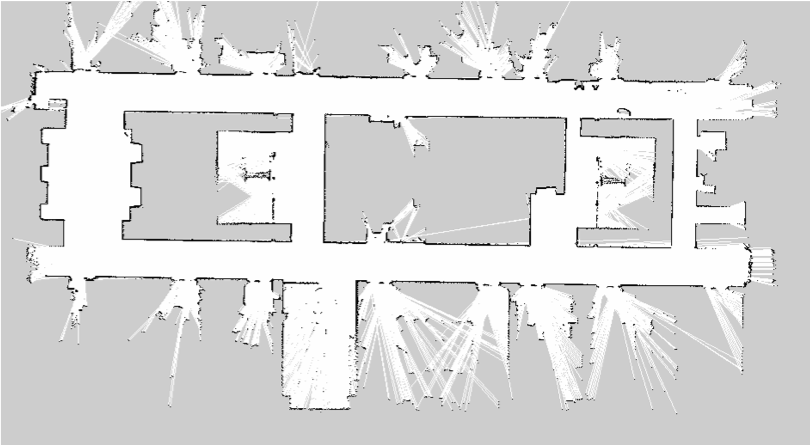
\includegraphics[width=12cm, ]{地図の障害物.png}
    \caption{Obstacles on the map}
    \label{fig:地図の障害物}
  \end{center}
\end{figure}

一方で, ロボットに搭載しているセンサにより, 障害物が直接観測できる必要はないものとする. 
しかし, 地図に載っている必要はあるため, SLAMにより地図を生成する場合, 
搭載したセンサにより観測ができないものについては, 手動等によって書き加えられている必要がある. 


%%%%%%%%%%%%%%%%%%%%%%%%%%%%%%%%%%%%%%%%%%%%%%%%%%%%%%%%%%%%%%%%%%%%%%%%%%%%%%%%
\section{価値反復による価値関数の計算} \label{section:価値関数}
本節では, 本手法および先行研究となるPFC法のオフラインフェーズである, 価値関数の計算について述べる. 
ロボットの観測の不確かさを考慮せず, 状態が既知であるという前提のもと, MDPを解くことで価値関数を計算する. 

%%%%%%%%%%%%%%%%%%%%%%%%%%%%%%%%%%%%%%%%
\subsection{状態空間の離散化}
計算機により価値関数$V$を計算するために, 状態空間の離散化が必要となる. 
状態空間$\mathcal{X}$を有限個の離散状態の集合$\mathcal{S}$で表現し, 
価値関数$V$は, この各離散状態に対する関数$V(\bm{s})$とする. 
このように, 離散化された状態空間における制御問題は, 有限マルコフ決定過程(finite Markov decision process, finite MDP)と呼ばれる. 

%%%%%%%%%%%%%%%%%%%%%%%%%%%%%%%%%%%%%%%%
\subsection{報酬} \label{subsection:報酬}
状態遷移に対する報酬について述べる. 
本論文では, 障害物がない通常の領域への状態遷移に対する報酬$r^{a}_{ss^{\prime}}$については, 状態遷移にかかる時間を$-\Delta t$とする. 
障害物内への状態遷移の報酬は, 障害物以外での状態遷移報酬に対し, 非常に小さい値とする. 

%%%%%%%%%%%%%%%%%%%%%%%%%%%%%%%%%%%%%%%%
\subsection{価値反復}
$S$に対する最適価値関数$V$は, 
\begin{equation}
\label{bellman equation}
  V(s) = \max_{a} \sum_{s^{\prime} \in \mathcal{S}}
         p^{a}_{ss^{\prime}} \left[ r^{a}_{ss^{\prime}} + V(s^{\prime}) \right]
\end{equation}
で計算することができ, この式はベルマン方程式と呼ばれる. 
計算をすべての離散状態$\mathcal{S}$に対して, 値が収束するまで繰り返し行っていくことで, 最適価値関数$V(s)$を求める. 
この方法は, 動的計画法のひとつである価値反復と呼ばれる. 
この価値反復により, 全離散状態$\mathcal{S}$に対する価値関数$V(s)$を事前に計算しておく. 


%%%%%%%%%%%%%%%%%%%%%%%%%%%%%%%%%%%%%%%%%%%%%%%%%%%%%%%%%%%%%%%%%%%%%%%%%%%%%%%%
\section{提案する手法} \label{section:回避重み}
本節では, パーティクル全体が障害物を回避するための方法について述べる. 
まず, 行動決定の際に行動を評価する式の変更, および追加するパラメータについて述べる. 
次に, 変数値の更新方法について述べる. 

%%%%%%%%%%%%%%%%%%%%%%%%%%%%%%%%%%%%%%%%
\subsection{回避用変数の導入}
本手法では, 各パーティクルが行動決定に与える影響を動的に変更させるために, 変数を追加で持たせる. 
パーティクル$\xi^{(i)}$は,  変数として状態$\bm{x}^{(i)}$と重み$w^{(i)}$を持っている. 
これに, 行動決定に与える影響を変更するためのパラメータ$m^{(i)}_{\rm avoid}$を追加で持たせる. 
変更後のパーティクルは, 
\begin{equation}
\label{particles}
  % \Xi_{t} = \{ \xi^{(i)}_{t} =
  %              (\bm{x}^{(i)}_{t}, w^{(i)}_{t}, m^{(i)}_{\rm avoid}) |i = 1,2,\dots,N \}
  \Xi = \{ \xi^{(i)} =
               (\bm{x}^{(i)}, w^{(i)}, m^{(i)}_{\rm avoid}) |i = 1,2,\dots,N \}
\end{equation}
のように定義される. 
$m^{(i)}_{\rm avoid}$の値は, $(m_{\rm avoid\_min} \leq m^{(i)}_{\rm avoid} \leq m_{\rm avoid\_max})$の範囲で変動する. 
なお, 変数$m^{(i)}_{\rm avoid}$は, 行動決定の際に用いるものであり, 自己位置推定においては使用されない. 

%%%%%%%%%%%%%%%%%%%%%%%%%%%%%%%%%%%%%%%%
\subsection{行動評価式の変更}
PFC法において, 行動を評価する式\ref{equation:pfc}は, 離散の状態空間$\mathcal{S}$では
\begin{equation}
\label{equation:finite pfc}
  Q_{\rm PFC}(a, b) = \sum_{i=1}^{N} \frac{ w^{(i)} }{ V(s^{(i)})^{m} }
                      \left[r^{a}_{s^{(i)} s^{\prime}} + V(s^{\prime}) \right]
\end{equation}
のように定義される. 
本手法では, この式を
\begin{equation}
\label{equation:modified pfc}
  % Q_{\rm PFC}(a, b) = \sum_{i=1}^{N} \frac{ w^{(i)} }{ V(s^{(i)})^{m} }
  %                     \left[r^{a}_{s^{(i)} s^{\prime}}
  %                           + V(s^{\prime})^{m^{(i)}_{\rm avoid}} \right]
  Q_{\rm PFC}(a, b) = \sum_{i=1}^{N} \frac{ w^{(i)} }{ V(s^{(i)})^{m} }
                      \left[r^{a}_{s^{(i)} s^{\prime}}
                            + V(s^{\prime}) \right] ^{m^{(i)}_{\rm avoid}}
\end{equation}
のように変更することで, $m^{(i)_{\rm avoid}}$の値により, パーティクルが行動に与える影響の大きさが変わるようにする. 

%%%%%%%%%%%%%%%%%%%%%%%%%%%%%%%%%%%%%%%%
\subsection{回避用変数値の更新} \label{subsection:回避用変数値の更新}
$m^{(i)}_{\rm avoid}$の更新方法について述べる. 
$m^{(i)}_{\rm avoid}$は, タスクの実行中, 状況に応じて
\begin{equation}
\label{equation:reward}
  m^{(i)}_{\rm avoid} =
  \left\{
    \begin{array}{l}
      m_{\rm avoid\_max} \ \ \ \ (r^{a}_{s^{(i)}s^{\prime}} < - \Delta t) \\
      m^{(i)}_{\rm avoid} \ \ \ \ ({\rm otherwise})
    \end{array}
  \right.
\end{equation}
のように更新する. 
行動評価のとき, あるパーティクルが行動$a$によって障害物に入る場合, 値を大きく増加させる. 
次ステップで障害物に入るという判断は, 報酬$r^{a}_{s^{(i)}s^{\prime}}$の値から判定することができる. 
\ref{subsection:報酬}節で述べたとおり, 本論文では, 報酬を式(\ref{equation:reward})の用に設定している. 
障害物外への状態遷移では, 報酬は$-\Delta t$となり, 障害物内への状態遷移では, それ以下となる. 
したがって, $m^{(i)_{\rm avoid}}$は, 
報酬が$-\Delta t$よりも小さくなる障害物内への状態遷移のときに, $m_{\rm avoid\_max}$へと更新し, 
障害物外への状態遷移では, $m^{(i)}_{\rm avoid}$の値は更新しない. 

%%%%%%%%%%%%%%%%%%%%%%%%%%%%%%%%%%%%%%%%
\subsection{回避用変数値の減衰}
更新した$m^{(i)}_{\rm avoid}$を, 時間とともに減少させる処理を加える. 
値の更新を\ref{subsection:回避用変数値の更新}項での処理のみで行った場合, ロボットの行動がループする可能性が考えられる. 
図\ref{fig:回避のループ}のに示すように, 障害物に衝突しそうなパーティクルが現れたとき, ロボットは回避動作を行う. 
しかし, 回避動作を行った直後, 次の行動で障害物に衝突しそうなパーティクルがなくなった場合, ロボットは再度ゴールへと向かう動作を行ってしまう. 
ロボットはゴールへと向かう動作と, 障害物回避の動作を交互に繰り返してしまい, 行動の停滞が起きてしまうことが考えられる. 
したがって, 一度障害物へと入りそうになったパーティクルとそれ以外のパーティクルで, 行動決定に与える影響に差ができる状況を一定時間継続させる必要がある. 
本論文では, 時間とともに線形に減少していく方法をとることとする. 
一度$m_{\rm avoid\_max}$まで増加した$m^{(i)}_{\rm avoid}$は, 10秒後に$m_{\rm avoid\_min}$になるように減衰させていく. 

\begin{figure}[h]
  \begin{center}
    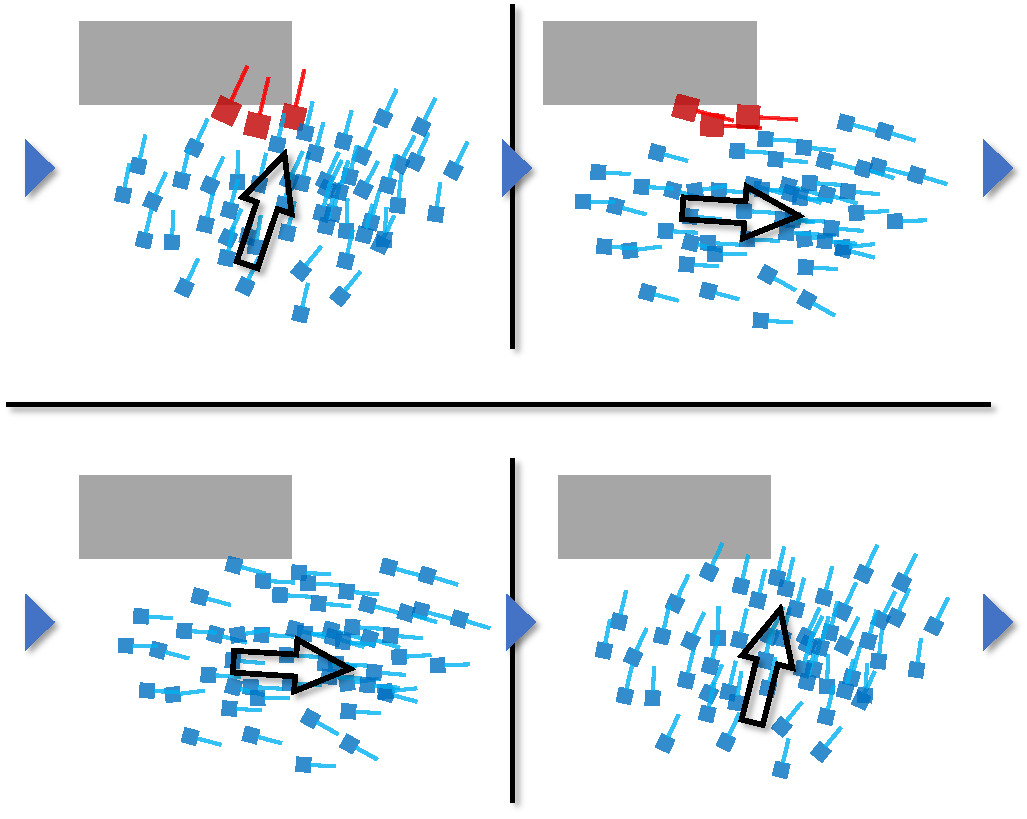
\includegraphics[width=12cm, ]{回避のループ.pdf}
    \caption{Action stagnation due to repeated avoidance behavior}
    \label{fig:回避のループ}
  \end{center}
\end{figure}
